\section{Vorstellung des Prototypen}\label{prototyp}
Der Prototyp demonstriert, wie eine Software entsprechend der in Kapitel \ref{wsk} aufgeführten Bausteine einem Fahrzeughalter bereitgestellt und von diesem genutzt werden kann. Konkret wird die Bereitstellung einer Software dargestellt, mit welcher \textbf{ein Fahrzeughalter ein Parkticket kaufen und das Fahrzeug anschließend selbstständig zum Parkplatz fahren kann.} Zunächst wird in Kapitel 5.1 dargestellt, wie der Prototyp installiert werden kann. Im Anschluss daran wird in Kapitel 5.2 die Software Architektur des Prototypen vorgestellt. Abschließend werden die Funktionen des Prototypen vorgestellt und wie diese genutzt werden können. 

\subsection{Architektur des Prototypen}	
Abbildung \hyperref[img:basic]{13} zeigt die Grundlegende Architektur des Prototypen. Der OEM-Server ist das Back-End des Shops und stellt die Single-Source-Of-Truth für Fahrzeuge dar. Der \textbf{Software Applikation Manager} \textit{(SAM)}, die \textbf{Mensch Maschine Schnittstelle} \textit{(MMS)} und die \textbf{Carla Simulation} bilden gemeinsam die Repräsentation des simulierten Fahrzeugs. Der Software Applikation Manager ist mit allen Modulen des Prototypen verbunden und stellt somit die zentrale Steuerungseinheit des Fahrzeugs dar. Über ihn erfolgt die Installation und die Nutzung von Softwares. Die Mensch Maschine Schnittstelle ist eine Android-Schnittstelle, auf welcher eine Version des Software Shops als App installiert ist. Über diese App können Nachrichten von dem Software Applikation Manager empfangen und verarbeitet werden und es können Nutzereingaben getätigt werden, durch welche der Ablauf der Simulation gesteuert werden kann. Alle Drei Module sind in Java implementiert worden. Die Python-basierte Carla Simulation ist die visuelle Repräsentation des Fahrzeugs und veranschaulicht getroffene Entscheidungen.
\begin{figure}[!h]
	\centering
	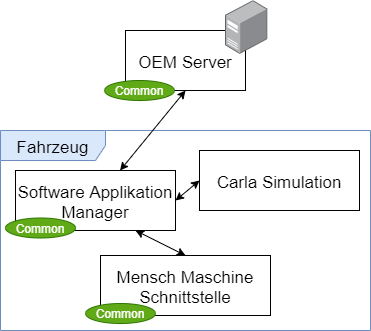
\includegraphics[width=0.5\columnwidth]{pictures/konzept-basic.png}
	\label{img:basic}
	\caption{Grundlegende Architektur der Prototypen}
\end{figure}

Der SAM, der Server und die MMS sind alle Java-basiert und kommunizieren auf Basis der \textbf{Common-Library} miteinander, welche in  \hyperref[img:common]{Abbildung 14} gezeigt wird. Sie ist eine Sammlung an Java-Objekten, welche für die Anwendungsfall-bezogene Kommunikation notwendig sind und daher jedem Modul bekannt sein müssen. Sie enthalten Primitive Werte \textit{(Integer, String, Long, etc.)} und leiten alle vom Serializable-Interface ab, damit sie über geschaffenen Netzwerkschnittstellen verschickt werden können. \\
Die Common-Objekte sind in zwei Gruppen unterteilt, die \textbf{Environment-Objekte} und \textbf{Messages}. Messages sind die Objekte, die im Prototypen zwischen den einzelnen Komponenten verschickt werden und so den Ablauf des Prototypen bestimmen. Sie beinhalten neben Primitiven Datentypen auch Environment Objekte und stellen die Basis der anwendungsfallbezogenen Kommunikation dar. Es wird zwischen SoftwareMessages und ServiceMessages unterschieden, wobei SoftwareMessages Nachrichten sind die zur Installation oder Nutzung einer Software benötigt werden und ServiceMessages sind jene, die zur Kommunikation mit einem Service Provider notwendig sind.
\begin{figure}[!h]
	\centering
	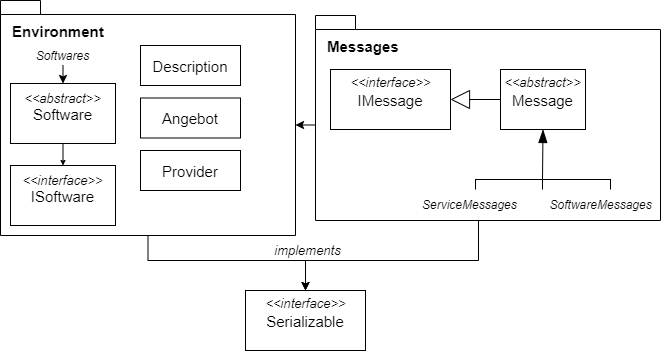
\includegraphics[width=0.8\columnwidth]{pictures/konzept-Common.png}
	\label{img:common}
	\caption{Aufbau der Common Library}
\end{figure}

Die in den Messages enthaltenen Environment-Objekte vereinfachen die Kommunikation der Module im Kontext des Anwendungsfalls. Die \textit{Description }wird verwendet, wenn eine Software oder ein Service von einer Nachricht beschrieben werden soll und das \textit{Provider}-Objekt ist dafür da, sowohl Software- als auch Service Provider einbeziehen zu können. Das Angebot-Objekt wird für die Bereitstellung von Auswahlmöglichkeiten beim Kauf einer Software wie zum Beispiel Kauf und Abo verwendet. Die abstrakte Klasse \textit{Software } ist die Elternklasse für Softwares, welche dem Prototypen neue Anwendungsfälle hinzufügen sollen. Jede neu hinzugefügte Software überschriebt die von dieser Klasse vorgegebene Methode \textit{handleMessage()}. Diese Methode wird im Prototypen aufgerufen, um Nachrichten von einer Services gemäß des Anwendungsfallkontexts zu verarbeiten. 

\subsubsection{Architektur des Software Applikation Managers (SAM)}
Wie zuvor erwähnt, wird über den Software Applikation Manager das Geschehen des Prototypen gesteuert. Er ist, wie in Abbildung \hyperref[img:sam]{15} zu sehen ist, in drei Module aufgeteilt: Die GUI ist die View-ebene des Prototypen, über welche das Geschehen der Simulation nachvollzogen und gesteuert werden kann. Die GUI wurde mit dem JavaFX-Framework erstellt und es wurde AfterburnerFX als weitere Unterstützung hinzugenommen. Durch AfterburnerFX wird das View-binding der einzelnen Elemente der GUI automatisiert und somit viel \glqq Boilerplate Code\grqq vermieden.\\
Im \textit{Car} befindet sich der MessageHandler, welcher die zentrale Steuereinheit des SAM ist. Er verbindet sich mit Hilfe der Klassen des \textit{Networks} mit dem Server und öffnet die Ports, mit welchen sich die MMS und die Carla-Simulation verbinden können. Über diese Schnittstellen eingehende Nachrichten werden auf einen EventBus gepostet, der sich im MessageHandler befindet. Hierdurch kann die Simulation auf die Nutzereingaben aus GUI und MMS reagieren und die Nachrichten getrennt voneinander behandeln. Für die Installation und Nutzung von Softwares wird der SoftwareManager genutzt, welcher alle installierten Softwares des Fahrzeugs verwalten und zum benötigten Zeitpunkt bereitstellen kann.
\begin{figure}[!h]
	\centering
	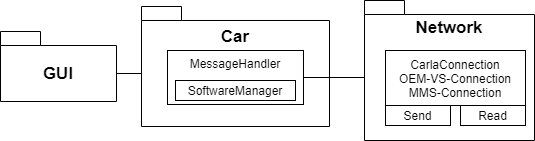
\includegraphics[width=0.8\columnwidth]{pictures/konzept-SAM.png}
	\label{img:sam}
	\caption{Architektur des Software Applikation Managers}
\end{figure}

\subsubsection{Architektur des OEM-Servers (Server)}
Die in Abbildung \hyperref[img:server]{16} dargestellte Architektur wurde nach der Vorlage des Uptane-Standards entworfen. Es wird eine Netzwerkverbindung mittels Netty\footnote{\url{https://netty.io/}} erstellt, mit welcher sich der SAM verbinden kann. Durch die Integration von Netty ist es möglich mehrere Software Applikation Manager mit dem Server zu verbinden, wodurch der Prototyp einfach skaliert werden kann. Über Netty eingehende Nachrichten werden auch hier wieder über einen EventBus an den Director weitergeleitet und von diesem verarbeitet. Der Director ist mit dem \textbf{Image Repository} verbunden, in welchem sich die Softwares befinden die im Shop verfügbar sind. Uptane gibt vor, zusätzlich eine \textbf{Inventory Database} zu führen in welcher die Manifeste aller im Shop registrierter Fahrzeuge in der Form gespeichert sind wie sie zuletzt von dem Director verifiziert wurden, \cite[Vgl. Abschnitt 5.3.2.2]{uptaneDoc} welcher daher auch hier integriert wurde. Wird eine Anfrage an den Server geschickt, vergleicht der Director das mitgeschickte Manifest mit dem in der Inventory Database gespeicherten Version. Werden Unterschiede oder sonstige Sicherheitslücken festgestellt, wird die Anfrage des Fahrzeugs für neue Software zurückgewiesen. \cite[Vgl. Abschnitt 5.3.2.1]{uptaneDoc}
 
\begin{wrapfigure}{R}{0.5\textwidth}
	\centering
	\includegraphics[width=0.48\textwidth]{pictures/konzept-OEM-vs.png}	
	\label{img:server}
	\caption{Architektur des Servers}
\end{wrapfigure}

\noindent
Der Director kann eingehende Anfragen an den Software-User-Pattern-Recognizer\textit{(SUPR)} weiterleiten, welcher in Kapitel \hyperref[fs]{zwei} vorgestellt wurde. Der SUPR ist dafür zuständig, den Software-Bedarf von Fahrzeughaltern anhand ihrer Fahrdaten zu bestimmen. Er hat ebenfalls Zugriff auf das Image Repository und das \textit{Scenario Repository} in welchem, wie in Kapitel \hyperref[konzept]{zwei} erwähnt, die zu einer Software hinzugefügten Szenarien gespeichert sind. Stellt der SUPR einen Softwarebedarf fest, wird dieser an den Director weitergegeben der infolgedessen  die entsprechende Software dem Fahrzeughalter vorschlägt.

\subsection{Installation}
Die Installation der einzelnen Module muss muss getrennt voneinander passieren. Für die vollständige Nutzung muss sichergestellt sein, dass Carla auf dem PC auf welchem der Prototyp installiert werden soll lauffähig ist. Schauen Sie hierzu in die Systemanforderungen von Carla.  \footnote{\url{https://carla.readthedocs.io/en/latest/start_quickstart}, Aufgerufen am \today} Der SAM und der Server müssen auf dem selben PC installiert werden, während die anderen Module können auch auf weiteren Geräten genutzt werden können. Hierzu müssen die IP-Adressen und Ports der Module über deren Config-Dateien angepasst werden. Wie dies getan werden kann und welche weiteren Schritte für die Installation befolgt werden müssen, stellt die folgende Anleitung dar. Sie ist für Windowsgeräte ausgelegt und dauert ca. 30-40 Minuten.


\subsubsection{Server und SAM Installation}
\begin{itemize}
	\item[\textbf{1.}] \textbf{.zip-Ordner Herunterladen}\\
	Gehen Sie auf \url{https://github.com/hesty98/bachelorthesis}. Klicken Sie auf den \textit{"releases"}-Tab, welcher unter der Beschreibung des Repository zu finden ist.
	Laden Sie die Datei \textit{"prototyp.zip"} herunter und entpacken Sie den Ordner auf ihrem Laptop. In diesem Ordner finden Sie die .jar-Dateien mit welchen der Server und der SAM gestartet werden können. Der Ordner \textit{"PythonScriptsThesis"} wird später für die Installation von Carla benötigt.
	
	\item[\textbf{2.}] \textbf{IP-Adresse aufschreiben}\\
	Um das MMS und auch Carla mit dem Software Applikation Manager zu verbinden, müssen Sie ihre IP-Adresse kennen. Öffnen Sie hierzu ihr Windows-Terminal und geben Sie \textit{ipconfig} ein. In der Zeile \glqq IPv4-Adresse\grqq steht ihre die IP-Adresse. Diese müssen Sie sich merken.
\end{itemize}


\subsubsection{MMS Installation}
\begin{itemize}
	\item[\textbf{1.}] \textbf{Android Studio herunterladen}\\
	Sie haben zwei Optionen, wie die Mensch Maschine Schnittstelle genutzt werden kann. Entweder sie simulieren das Android Gerät auf ihrem PC oder Sie installieren die App auf ein eigenes Tablett/Smartphone. Für beides wird eine aktuelle Version von Android Studio benötigt, die Sie hier (\url{https://developer.android.com/studio}) herunterladen können. Installieren Sie Android Studio und fahren Sie anschließend vor.

	\item[\textbf{2.}] \textbf{Code importieren}\\
	Das Repository der Mensch Maschine Schnittstelle liegt auf GitHub. Über Android Studio können Sie das Projekt direkt importieren. Klicken Sie hierfür auf \glqq File\grqq -> \glqq new\grqq -> \glqq Project from Version control\grqq -> \glqq Git\grqq und geben sie folgende URL ein: \url{https://github.com/hesty98/HMI.git}.	Alternativ kann das Projekt auch als .zip-Datei Heruntergeladen werden. Der extrahierte Ordner kann in Android Studio als Projekt geöffnet werden \textit{(\glqq File\grqq -> \glqq open\grqq -> \glqq Ordner wählen\grqq)}.
	
	\item[\textbf{3.}] \textbf{MMS Konfigurieren}\\
	Öffnen Sie in Android Studio die Datei Connection.java und passen Sie den Host entsprechend der IP des \textit{Software Applikation Managers} an. Die Datei befindet sich im 'network'-Ordner \textit{(app -> java -> com.linushestermeyer.hmi -> network)}.
	
	\item[\textbf{4.}] \textbf{MMS aufsetzen}\\
	Sie können die Mensch Maschine Schnittstelle nun entweder auf einem eigenen Gerät installieren oder das Gerät auf ihrem PC simulieren. Für beide Optionen müssen Sie zuerst eine Konfiguration für die App erstellen.  Folgen Sie hierzu folgender Anleitung: \url{https://developer.android.com/studio/run/rundebugconfig}.
	
		\subitem \textbf{4.1 Eigenes Tablet/Smartphone}\\
			Zur Installation auf einem eigenen Gerät müssen Sie zunächst die \textit{Entwickler-Optionen} für dieses Freischalten und \textit{USB-Debugging} aktivieren. Folgen sie hierfür folgender Anleitung: \url{https://mobilsicher.de/ratgeber/usb-debugging-aktivieren}. Wurde dies getan, kann das Gerät an den PC angeschlossen werden. Über den grünen 'Play'-Button in der oberen Menuleiste kann die App auf Ihrem Gerät installiert werden.
			
		\subitem \textbf{4.2 Virtual Device}\\
			Wenn Sie Die App \textbf{nicht} auf einem eigenen Gerät installieren wollen, müssen sie mit Android Studio ein Simuliertes Gerät erstellen. Dies funktioniert nur, wenn ihr PC eine \textbf{Intel-CPU} hat, da Android Studio den \textit{HAXM-Service} von Intel zur Simulation nutzt. Ist dies der Fall, können Sie mit Hilfe folgender Anleitung ein Virtuelles Gerät erstelle: \url{https://developer.android.com/studio/run/managing-avds}. Erstellen Sie eine Instanz eines Tablets nicht die eines Smartphone, damit die Benutzeroberfläche der MMS gut dargestellt wird. \\
			Haben Sie ein \textit{VD} erstellt, können sie anschließend über den grünen 'Play'-Button in der oberen Menuleiste die App auf diesem Gerät installieren. 
\end{itemize}


\subsubsection{Carla Installation}
\begin{itemize}
	\item[\textbf{1.}] \textbf{Python installieren und SYS\_PATH hinzufügen}\\
	Damit Carla auf dem PC laufen kann, muss Python in Version 3.7 auf dem PC installiert sein und dem SYSTEM\_PATH hinzugefügt werden. Hierzu kann folgende Anleitung genutzt werden, wobei die \glqq 3.4\grqq durch eine \glqq 3.7\grqq zu ersetzen ist: \url{https://geek-university.com/python/add-python-to-the-windows-path/}. Der SYSTEM\_PATH kann bei der Installation auch durch das ankreuzen einer Checkbox automatisch gesetzt werden.
	
	\item[\textbf{2.}] \textbf{Carla Herunterladen}\\
	Carla kann als .zip-Ordner hier (\url{https://github.com/carla-simulator/carla/blob/master/Docs/download.md}) Heruntergeladen werden - nutzen Sie die Version 0.9.7 . Die Dateien müssen in einen eigenen Ordner auf dem PC extrahiert werden. Nun müssen die für die Simulation notwendigen  Python-Packages \textit{pip, pygame und numpy} installiert werden. Die pip-Installation kann hier nachgelesen werden: \url{https://pypi.org/project/pip/}. Für die Installation von pip sollte die Administrator-Konsole verwendet werden. Suchen Sie hierzu im Windows Suchbalken nach \glqq cmd\grqq und führen sie das Terminal mittels eines Rechtsklick \glqq als Administrator aus \grqq. Die Installation von pip muss im 'PythonAPI'-Ordner des Carla-Downloads erfolgen, daher müssen sie in der Konsole in diesen Ordner wechseln \textit{(cd ..Pfad/Von/Carla/.../PythonAPI.)} Ist pip installiert, können mittels folgender Zeile die übrigen packages hinzugefügt werden:
	\begin{verbatim}
	py -3.7 -u pip install --user pygame numpy 
	\end{verbatim}
	Im Anschluss daran sollten Sie Carla ein mal testen. Starten Sie zunächst die Carla.exe und wechseln sie im Terminall in den PythonAPI/examples Ordner \textit{(cd PythonAPI/examples)}. Führen Sie anschließend folgenden Befehl durch:
	\begin{verbatim}
	py -3.7 spawn_npc.py
	\end{verbatim}
	Klappt dies nicht, haben Sie bei der Installation einen Fehler gemacht. Überprüfen Sie, ob die benötigten Python-Packages installiert sind und gehen Sie sicher, dass Python in der Version 3.7 dem SYSTEM\_PATH hinzugefügt wurde.
	\item[\textbf{3.}] \textbf{Skripte einfügen}\\
	In der extrahierten .zip-Datei des SAM und Servers befindet sich ein Ordner mit dem Namen \textit{CarlaScriptThesis}. Kopieren Sie diesen Ordner in den \textit{PythonAPI}-Ordner von Carla und Sie haben es geschafft! 
	\item[\textbf{4.}] \textbf{Carla Konfigurieren}\\
	Abschließend sollten sie noch Konfigurationen an Carla vornehmen. Zunächst wird die Stadt geändert in welcher sich das Szenario abspielen wird. Öffnen Sie hierzu die \glqq DefaultEngine.ini \grqq Datei aus dem Ordner \grqq CarlaUE4/Config\glqq und ersetzen Sie \textit{Town0X.Town0X} überall mit \textit{Town02.Town02}. Löschen Sie die anderen Zeilen \textbf{nicht!}
	\begin{verbatim}
	EditorStartupMap=/Game/Carla/Maps/Town02.Town02
	GameDefaultMap=/Game/Carla/Maps/Town02.Town02
	ServerDefaultMap=/Game/Carla/Maps/Town02.Town02
	TransitionMap=/Game/Carla/Maps/Town02.Town02
	\end{verbatim}	
	Haben Sie die entsprechenden Werte eingetragen, speichern und schließen Sie die Datei. Anschließend wechseln sie in den Ordner \textit{PythonAPI/CarlaScriptThesis} und editieren Sie die simulation\_handler\_automatic.py. Passen Sie die IP im Skript an die des \textbf{Software Applikation Managers} an. 
\end{itemize}

\subsection{Nutzung des Prototypen}
Die Module des Prototypen müssen in bestimmter Reihenfolge gestartet werden. Öffnen Sie  zunächst zwei Terminals im heruntergeladenem Ordner und eines \textit{CarlaScriptThesis}-Ordner.
\begin{itemize}
	\item[\textbf{1.}]\textbf{Server starten}
	\begin{verbatim}
	java -jar Server.jar
	\end{verbatim}
	\item[\textbf{2.}]\textbf{Software Applikation Manager}\begin{verbatim}java -jar SAM.jar\end{verbatim}
	\item[\textbf{3.}]\textbf{Carla\\}
	Starten Sie die CarlaUE4-Anwendung. Führen Sie anschließend im Terminal im Ordner \textit{\glqq PythonAPI/CarlaScriptThesis\grqq} das Skript  simulation\_handler\_automatic.py aus.
	\begin{verbatim}
	py -3.7 simulation\_handler\_automatic.py
	\end{verbatim} 
	\item[\textbf{4.}]\textbf{Mensch Maschine Schnittstelle}\\
	Starten Sie die App auf ihrem Gerät oder in dem Virtual Device. Gehen Sie sicher, dass die App zuvor geschlossen war.
\end{itemize}
Im folgenden haben Sie fünf Bildschirme, über die alle Module des Prototypen sichtbar sind. Die Mensch Maschine Schnittstelle wartet auf eingehende Nachrichten, ebenfalls wie Carla. Die GUI des Software Applikation Managers ist in drei Bereiche aufgeteilt. Der Log auf Linken Seite stellt alle Ereignisse aus Sicht des Fahrzeugs dar. Der Log auf der Rechten Seite der GUI stellt sämtliche Ereignisse dar, die von dem Parkautomaten wahrgenommen werden. In der unteren rechten Ecke sind diverse Knöpfe zu sehen mittels welcher der Prototypen gesteuert werden kann - Abbildung 17 zeigt einen Screenshot dieser. In der Carla Simulation können Sie die Kamera mit Hilfe der WASD-Tasten und der Maus bewegen. Wenn Sie sich geradeaus und dann links bewegen, kommen sie zu dem 'Parkplatz'.
\begin{figure}[H]
	\centering
	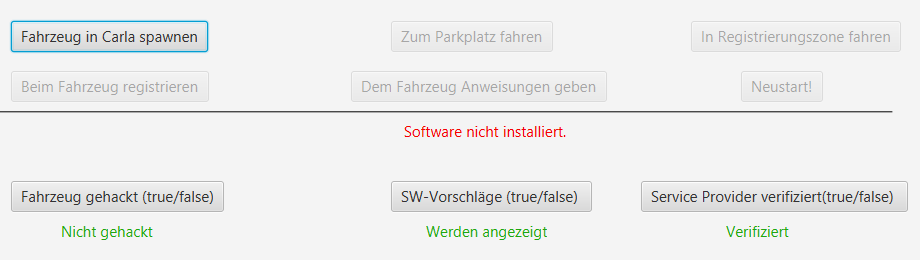
\includegraphics[width=\columnwidth]{pictures/gui_steuerung.PNG}
	\label{img:gui}
	\caption{Steuerung des Prototypen über die GUI}
\end{figure}

Über die oberen Knöpfe wird der Ablauf der Simulation gesteuert. Es ist immer nur möglich einen einzelnen Knopf zu bestätigen, die restlichen sind verblasst.\\\\
\textbf{Fahrzeug in Carla spawnen} Bei Bestätigung des Knopfes wird ein Fahrzeug in Carla gespawnt. Dies kann je nach Netzwerkgeschwindigkeit ein wenig dauern.\\
\\
\textbf{Zum Parkplatz fahren} Bei Bestätigung des Knopfes fährt das Fahrzeug geradeaus in Richtung des Parkplatzes und hält vor diesem.\\
\\
\textbf{In Registrierungszone fahren} Bei Bestätigung des Knopfes fährt das Fahrzeug in die \textit{Registrierungszone} des Parkplatzes und hält in dieser an.\\
\\
\textbf{Beim Fahrzeug registrieren} Bei Bestätigung des Knopfes schickt der Service Provider \textit{(Parkautomat)} eine Nachricht an das Fahrzeug. Die Nachricht wird im Log dargestellt und über die Mensch-Maschine-Schnittstelle kann auf diese reagiert werden. \\
\\
\textbf{Dem Fahrzeug Anweisungen geben} Bei Bestätigung des Knopfes wird dem Fahrzeug ein Anweisung gegeben, wohin es fahren soll. Entweder das Fahrzeug entfernt sich vom Parkplatz oder es parkt auf diesem.\\
\\
\textbf{Neustart} Bei Bestätigung des Knopfes wird das Fahrzeug von der Karte entfernt und die Simulation kann erneut durchgeführt werden.\\
\\
Die unteren Knöpfe bieten die Möglichkeit die Simulation anderweitig zu beeinflussen. Der in Rot dargestellte Indikator \textit{\glqq Software nicht installiert\grqq} gibt an, ob die Parksoftware bereits installiert ist oder nicht.\\
\\
\textbf{Fahrzeug gehackt} Bei Bestätigung des Knopfes wird das Manifest des Fahrzeugs geändert \textit{(\glqq gehackt\grqq)}. Wenn die Software noch nicht installiert ist (sie Indikator), kann sie auch dann nicht installiert werden weil das der Server die Installationsanfrage zurückweist. Die erneute Bestätigung des Knopfes macht dies rückgängig.\\
\\
\textbf{SW-Vorschläge} Bei Bestätigung des Knopfes wird verhindert, dass auf der MMS Softwares vorgeschlagen werden. Das erneute bestätigen macht dies rückgängig. Dies soll die Funktionalität eines \textit{Fahrzeug-basierten SUPR} darstellen.\\
\\
\textbf{Service Provider verifiziert} Die Bestätigung des Knopfes hat zur Folge, dass der Parkservice nicht mehr genutzt werden kann da der Service Provider nicht verifiziert ist. Das erneute bestätigen macht dies rückgängig.\\
\\
Auf der Mensch-Maschine-Schnittstelle werden PopUps angezeigt, wenn eine Software installiert oder ein Service genutzt werden soll. In diesen Popups kann ein Angebot ausgewählt werden und der Kauf/die Nutzung von Services und Softwares akzeptiert oder abgelehnt werden. Es sind die Grundlagen implementiert, die es künftige erlauben den Shop auch als solchen zu nutzen - diese haben in der Arbeit jedoch keinen weiteren Einfluss mehr gefunden.

\subsection{Analyse des Prototypen und Ausblick auf die Weiterentwicklung}
Im Prototypen wurde die im Forschungsseminer erläuterte Uptane Architektur versucht grundlegend zu implementieren. Hierdurch konnte gezeigt werden, wie ein Fahrzeug in der Zukunft von externen Eingriffen geschützt und die Sicherheit so gewährleistet werden kann. Der Prototyp hat dargestellt, wie eine Software über eine kabellose Schnittstelle orts- und zeitunabhängig gekauft und installiert werden kann. Zusätzlich wurde die Interaktion mit Service Providern veranschaulicht. Über die GUIs kann nachvollzogen und gesteuert werden, was in der Simulation passieren sollen. Die visuelle Repräsentation des Fahrzeugs in Carla unterstützt die Wirkung des Prototypen enorm, da der Betrachter direkt die Auswirkungen seiner Entscheidungen sieht. Auch die Interaktion über die Android-basierte Mensch Maschine Schnittstelle hat sich als sinnvoll erwiesen, da hierdurch ein guter Bezug zur Realität und Android Automotive gezogen werden kann. \\

Die erstellte Software Architektur lässt eine einfache Erweiterung des Prototypen zu. Für einen neuen Anwendungsfall muss lediglich eine neue Software erstellt werden und das Carla Skript muss angepasst werden was in geringer Zeit möglich ist. Die Nachrichten \textit{(Messages)} wurden generisch gehalten, damit sie künftig für neue Anwendungsfälle verwendet werden können.\\

Ein Bug, der sich nicht ohne weiteres beheben lies, ist die Dysfunktion des Carla-Skripts auf unterschiedlichen Computern. Der Bug ist, dass das Fahrzeug in Carla auf unterschiedlichen Computern unterschiedlich schnell fährt und lenkt, wodurch nicht immer der Parkplatz erreicht werden kann. Um den Prototypen dennoch komplett sehen zu können, wurde ein Video auf YouTube hochgeladen: \url{https://www.youtube.com/channel/UCO2segbDQ5BnGwshmWXeRcA}\\

Der Prototyp bietet noch eine Vielzahl an Erweiterungsmöglichkeiten. Der \textbf{Server} könnte um weitere Uptane-Funktionen erweitert werden und durch die Erstellung eines Server-seitigen SUPR wird die Möglichkeit geschaffen Suchalgorithmen wie sie im Laufe der Arbeit vorgestellt wurden in den Prototypen zu integrieren. Auch der \textbf{Software Applikation Manager} kann durch diverse neue Funktionen Sinnvoll erweitert werden. So kann ein Fahrzeug-basierter SUPR, dargestellt in Kapitel \ref{3.3}, bestimmen wann ein PopUp auf der MMS erscheinen soll und so das wahllose erscheinen von Softwarevorschlägen verhindern, was aktuell über den \textbf{SW-Vorschläge}-Knopf getan wird. Die Steuerung über die GUI sollte den neuen Anwendungsfällen entsprechend angepasst werden, da nicht in jedem Anwendungsfall eine Kommunikation mit einem Service Provider stattfindet. Die erstellten Knöpfe könnten auch generiert werden, wenn dem Prototypen ein \glqq Anwendungsfall\grqq-Objekt hinzugefügt wird, anhand wessen sich die GUI anpassen wird.  Entfernt man sämtliche Nutzereingaben des Prototypen und automatisiert so die gesamte Simulation, können die implementierten Anwendungsfälle beliebig hoch skaliert werden, wodurch die Zuverlässigkeit des Shops getestet werden könnte.\\

Im Laufe der Entwicklung wurde deutlich, dass Carla äußerst umfangreich ist. Würden die Funktionen von Carla ausgereizt werden, könnte eine Vielzahl neuer Anwendungsfälle zum Prototypen hinzugefügt und in Carla visuell dargestellt werden. Auch ein Wechsel zwischen autonomen Fahrfunktionen und eigenständiger Steuerung des Fahrzeugs kann in Carla erfolgen. Im aktuellen Prototypen ist Carla nur eine visuelle Repräsentation, wodurch eine zusätzliche Kommunikationsebene entsteht und die Laufzeit des Prototypen verschlechtert wird. Durch eine Implementierung des SAM in Python kann dies verbessert werden und die Architektur kann um ein Modul verkleinert werden, was auch die Installation erleichtern würde. Carla wäre dadurch sowohl die visuelle Repräsentation des Fahrzeugs als auch die "Business Logik".